\question 一主机的Cache容量是256块,采用全相联映射方式,主存中的第i块将会映射到Cache的第(
)块
\par\twoch{256}{i(mod 256)}{i}{\textcolor{red}{任何一块}}
\begin{solution}D。 全相联映射允许主存中的每个字块映射到Cache中的任何一块的位置上。
\end{solution}
\question 假设主存按字节编址,Cache共有64行,采用直接映射方式,主存块大小为32字节,所有编号都从0开始。现已知主存第3000号单元现在Cache中,那么其所在Cache的行号为
\par\twoch{13}{26}{\textcolor{red}{29}}{58}
\begin{solution}C。 i=jmodC
其中,i为Cache的行号,j为主存中的块号,C为Cache的块数(行数)。
现已知C=64,只需要求得j即可。
主存第3000号单元,即第3000B,又一个主存块为32B,3000/32=93余24,故其在第94块上,又编号从0开始,即在编号为93的块中。
i=93mod64=29,故本题选C。 【本题扩展】
若把``直接映射方式''改为``4路组相联映射方式'',那么其Cache的组号为多少?
i=jmodC 其中,i为Cache的组号,j为主存中的块号,C为Cache的组数。
j的求解同上:主存第3000号单元,即第3000B,又一个主存块为32B,3000/32=93余24,故其在第94块上,又编号从0开始,即在编号为93的块中。
Cache有64行,一组有四行,则Cache有64/4=16组,即C=16。
那么i=93mod16=13,即其Cache的组号为13。
\end{solution}
\question 某计算机的Cache和主存的映射方式采用组相联映射方式,且采取分页管理存储方式,页面大小为128B,Cache容量为64页,按4页分组,主容量为4096页。那么主存地址的位数为(
)。【按字节寻址】
\par\twoch{12}{18}{\textcolor{red}{19}}{20}
\begin{solution}C。 本题有较多干扰条件,基础不扎实的同学容易受到误导。
主存地址,只跟主存总容量,和寻址单位相关。
主存总容量为4096×128B=2\^{}19B。又寻址单位一般默认为字节。则主存中单元数为2\^{}19。则主存地址的位数为19。
\end{solution}
\question 有一个主存---Cache层次的存储器,主存容量为1MB,Cache容量为64KB,每块8KB,采用直接映射方式,若主存地址为25301H,那么它映射到Cache的块号为(
)。【块号从0开始,按字节编址】
\par\twoch{1}{\textcolor{red}{2}}{3}{4}
\begin{solution}B。 主存地址有20位,
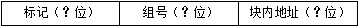
\includegraphics[width=3.73958in,height=0.28125in]{computerassets/8897229bdfb39d439c35ffdad2d4769f.jpeg}
首先块内地址位数为log2(8KB/1B)=13。 组号位数为log2(64KB/8KB)=3。
标记位数为20-13-3=4位。 那么25301H改写为二进制地址如下图所示:
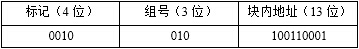
\includegraphics[width=3.73958in,height=0.51042in]{computerassets/d5c9ffa1a1c8153dee0b8c0ff80f238c.jpeg}
也就是说,映射到Cache的第2块。(块号从0开始)
\end{solution}
\question 已知Cache
A采用直接映射方式,共16行,块大小为1个字节,缺失损失为8个时钟周期;CacheB也采用直接映射方式,共4行,块大小为4个字节,缺失损失为11个时钟周期。假设开始时Cache为空,按照字节寻址,那么下列访问地址序列中,CacheB`具有更低的缺失率,但CacheB的总缺失损失反而比CacheA大的是
\par\twoch{1,2,3,4}{\textcolor{red}{0,2,4,8,0}}{0,1,0,1,0,1}{0,8,0,8,0,8}
\begin{solution}B。 设Cache A和Cache B的缺失次数分别为
a和b,根据题目最后的要求a和b就必须满足:
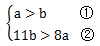
\includegraphics[width=1.04167in,height=0.47917in]{computerassets/f5fe4befaad7c28dbc80b0c430cfe843.jpeg}
选项A中,1,2,3,4,CacheA缺失4次,而Cache B缺失2次,不满足②。
选项B中,0,2,4,8,0,CacheA缺失4次,而CacheB缺失3次,满足①和②。
选项C中,0,1,0,1,0,1,CacheA缺失2次,而CacheB缺失1次,不满足②。
选项D中,0,8,0,8,0,8,CacheA缺失2次,而CacheB缺失2次,不满足①。
综上所述,本题选B。
\end{solution}
\question 某一计算机采用主存---Cache存储层次结构,主存容量有8个块,Cache容量有4个块,采取直接映射方式。若主存块地址流为0、1、2、5、4、6、4、7、1、2、4、1、3、7、2,一开始Cache为空,此期间Cache的命中率为
\par\twoch{13.3\%}{20\%}{\textcolor{red}{26.7\%}}{33.3\%}
\begin{solution}C。 在直接映射方式中,存储块都唯一映射到一个Cache映像块中。
Cache块号=主存块号 mod Cache块数。
于是,每次访问后,Cache中存放的主存块情况如下图所示:
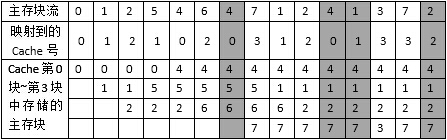
\includegraphics[width=4.65625in,height=1.45833in]{computerassets/9555ff92dfec9b27551485a6ff8fd8cd.jpeg}
底纹为灰色的部分,为命中时刻。即有4次命中,那么命中率为4/15=26.7\%。故本题选C。
\end{solution}
\question (清华大学)某计算机的Cache---主存层采用组相联映射方式,页面大小为128字节,Cache容量为64页,按4页分组,主存容量为4096页,按字节编址,那么主存储器地址共需(
)位
\par\twoch{\textcolor{red}{19}}{18}{20}{以上都不对}
\begin{solution}A。 主存容量=4096×128字节=219字节,所以主存地址共需19位。
\end{solution}
\question (西安电子科技大学,2007年)某存储系统中,主存容量是Cache容量的4096倍,Cache被分为64个块,当主存地址与Cache地址采用直接地址变换时,主存变换表的大小应为(
)(假设地址变换表每行仅存储主存字块标记)
\par\twoch{6×12bit}{6×4096bit}{\textcolor{red}{64×12bit}}{64×4096bit}
\begin{solution}C。
Cache被分为64个块,故地址变换表为64行,每行存储主存字块标记为12位(2\^{}12=4096)。
\end{solution}
\question 主存与Cache间采用全相联映射方式,Cache容量4MB,分为4块,每块1MB,主存容量256MB。若主存读/写时间为30ns,Cache的读/写时间为3ns,平均读/写时间为3.27ns,则Cache的命中率为
\par\twoch{90\%}{95\%}{97\%}{\textcolor{red}{99\%}}
\begin{solution}D。 此题属于逆向解题,没有出过类似的题目,考生需引起重视。
根据公式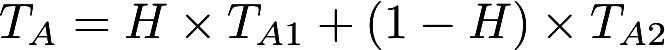
\includegraphics[width=2.37500in,height=0.18750in]{texmath/9082595Cdpi7B3507D7BT_A7D3DH5Ctimes7BT_7BA17D7D2B281-H295Ctimes7BT_7BA27D7D},可求得Cache的命中率为99\%。
解题技巧:题干中真正有意义的数据是主存读/写时间、Cache的读/写时间和平均读/写时间,据此就可以求出Cache的命中率,其他数值在求解中都没有用,属于干扰数据。
\end{solution}
\question 关于Cache的3种基本映射方式,下面叙述中错误的是
\par\fourch{Cache的地址映射有全相联、直接、多路组相联等3种基本映射方式}{全相联映射方式,即主存单元与Cache单元随意对应,线路过于复杂,成本太高}{多路组相联映射是全相联映射和直接映射的一种折中方案,有利于提高命中率}{\textcolor{red}{直接映射是全相联映射和组相联映射的一种折中方案,有利于提高命中率}}
\begin{solution}D。
Cache存储器通常使用3种地址映射方式,它们是全相联映射、直接映射、多路组相联映射方式。
1)全相联映射方式,主存单元与Cache单元随意对应,有最大的使用灵活性,但地址标志字段位数多,比较地址时可能要与所有单元比较,线路过于复杂,成本太高,只用于Cache容量很小的情况。
2)直接映射方式,一个主存单元只与一个Cache单元硬性对应,有点死板,影响Cache容量的有效使用效率,即影响命中率,但地址比较线路最简单,比较常用。
3)多路组相联映射方式,一个主存单元可以与多个Cache单元有限度地随意对应,是全相联映射和直接映射的一种折中方案,有利于提高命中率,地址比较线路也不太复杂,是比较好的一种选择。
\end{solution}
\question 容量为64块的Cache采用组相联映射方式,字块大小为128个字,每4块为一组。如果主存为4K块,且按字编址,那么主存地址和主存标记的位数分别为
\par\twoch{16,6}{17,6}{18,8}{\textcolor{red}{19,8}}
\begin{solution}D。
因为主存容量4K×128=512K字,所以主存地址19位。又因为字块大小为128个字,所以块内地址7位,Cache被分成64/4=16组,故组号4位,主存标记19-4-7=8位。
归纳总结:主存地址由主存标记、组号和块内地址3部分组成。
解题技巧:首先算出主存的容量,得出主存地址的位数,然后根据组相联方式和块的大小,确定组号字段的位数和块内地址字段的位数,即可得出主存标记的位数。
\end{solution}
\question Cache用组相联映射,一块大小为128B,Cache共64块,4块分一组,主存有4096块,主存地址共需(
)位
\par\twoch{\textcolor{red}{19}}{18}{17}{16}
\begin{solution}A。
主存有4096块,每块大小128B,则主存容量共有4096×128B=512KB,共需地址线19位。
解题技巧:此题在计算时,只需要算出主存的容量即可得出结果,实际上与采用什么映射方式没有关系,不需要考虑组相联的问题。另外,还需要知道Cache的块大小和主存的块大小是一样大的,不然此题也无法作答。
\end{solution}
\question 有效容量为128KB的Cache,每块16B,8路组相联。字节地址为1234567H的单元调入该Cache,其tag应为
\par\twoch{1234H}{2468H}{\textcolor{red}{048DH}}{12345H}
\begin{solution}C。
因为块的大小为16B,所以块内地址字段为4位;又因为Cache容量为128KB,8路组相联,所以可以分为1024组{[}128KB/(8×16B)=1024{]},对应的组号字段10位;剩下为标记字段。1234567H=0001001000110100010101100111,标记字段为其中高14位,00010010001101=048DH。
归纳总结:组相联映射对应的主存地址应包括3部分:标记(Tag)、组号(Index)和块内地址(Offset)。
解题技巧:首先将主存地址由十六进制变成二进制,其中块内地址字段为最后4位,组号字段为中间10位,剩下的就是标记字段,将标记字段二进制转换为十六进制,即可得出结果。
\end{solution}
\question 假设某计算机按字编址,Cache有4个行,Cache和主存之间交换的块大小为1个字。若Cache的内容初始为空,采用2路组相联映射方式和LRU替换算法,当访问的主存地址依次为0,4,8,2,0,6,8,6,4,8时,命中Cache的次数是(
)
\par\twoch{1}{2}{\textcolor{red}{3}}{4}
\begin{solution}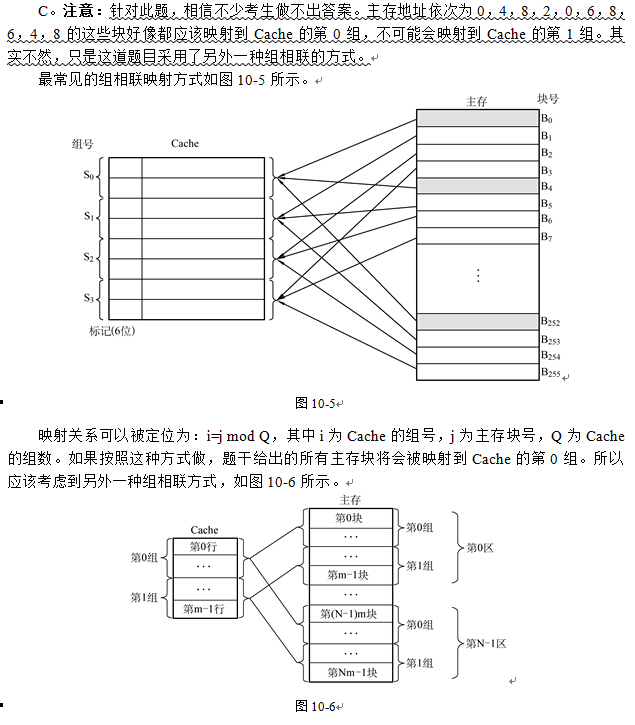
\includegraphics[width=6.61458in,height=7.55208in]{computerassets/ff0c95e262008e1450dfd6e70ac0cf03.jpeg}
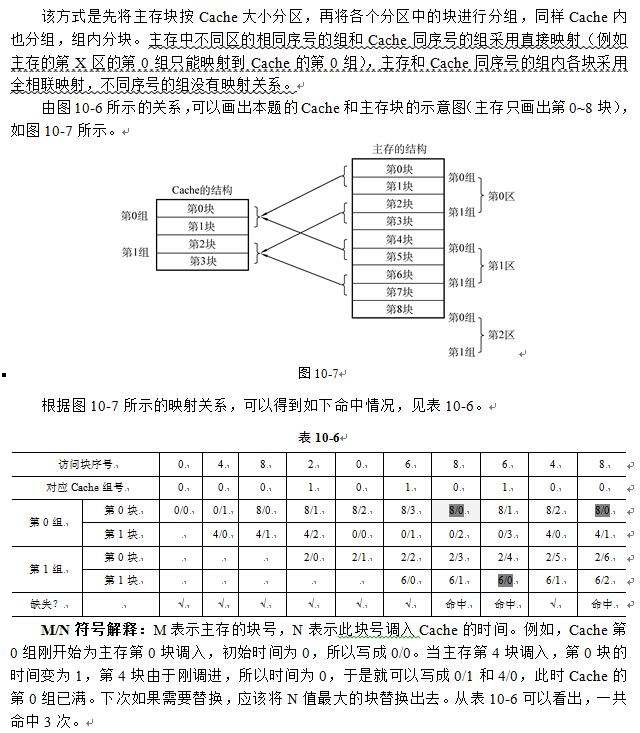
\includegraphics[width=6.66667in,height=7.63542in]{computerassets/3f06ac0859d8a5c827fb5e5c108f981b.jpeg}
\end{solution}
